\documentclass[a4paper, 12pt]{article}
\usepackage{amsmath}
\usepackage{amsthm}
\usepackage{amssymb}
\usepackage{longtable}
\usepackage{pdflscape}
\usepackage{algorithm}
\usepackage{graphicx}
\usepackage[noend]{algpseudocode}
\usepackage{url}
\usepackage{tikz}

\newlength\tindent
\setlength{\tindent}{\parindent}
\setlength{\parindent}{0pt}
\renewcommand{\indent}{\hspace*{\tindent}}

\newtheorem{thm}{Theorem}
\newtheorem{cor}{Corollary}[thm]
\newtheorem{lemma}{Lemma}[thm]

\title{COMP 307 Assignment 2}
\author{Daniel Braithwaite}

\begin{document}
	\pagenumbering{gobble}
	\maketitle
	\newpage
  	\pagenumbering{arabic}
  	
	\section{Neural Network for Classification}
		\subsection{Network Architecture}
			For this problem the number of input nodes is 4 as there are 4 features and the number of output nodes is 3 as there are three possible classes for each instance.
			
			I started with 1 hidden layer as this is all you should need for a problem. As for the number of hidden nodes I started with 1 and kept adding 1 until it wasn't making a difference to the performance. Following this I ended up with 6 hidden nodes.
			
			\begin{center}
				\includegraphics[scale=0.5]{network}
			\end{center}
		
		\subsection{Learning Parameters}
			First to decide the learning rate I started at 0.2 and observed the error graph to find where to stop changing it.
			
			\begin{center}
				\includegraphics[scale=0.5]{training-error}
			\end{center}
			
			In the graph above the black line is with a learning rate of 0.2, then the blue is 0.3, red is 0.4, green is 0.5 and the last one is 0.6. My final learning rate was 0.5 as this converged just a little faster than 0.6.
			
		\subsection{Termination Criteria}
			Another observation which can be made from the graph above is that 100 iterations is far to many. The network converges quickly in under 10 best case and 20 worst case. For this reason the termination criteria are either a perfect solution or after 30 iterations.			
			
		\subsection{Results}
		
		\subsection{Comparison To Nearest Neighbor}
  	
  	\section{Genetic Programming for Symbolic Regression}
  	
  		\subsection{Terminal Set}
  			For this problem I chose the following two terminal nodes
  			
  			\begin{enumerate}
  				\item \textbf{Current X:} We want to find a function for Y in terms of X so we need to be able to include X in the function
  				
  				\item \textbf{Random Number:} The function for Y might not be only in terms of X, it could also include constant values which is why we need to include random constant numbers.
  			\end{enumerate}

		\subsection{Function Set}
			I started with a basic set of functions, these being \textbf{+}, \textbf{-}, \textbf{*} \textbf{/} (protected division). I chose this set as it is the minimal set of functions needed to construct a curve in the plane. After running the GP it gave a near perfect solution (which had an error of $1.4*10^-10$) so I was able to conclude that no extra functions where needed.
			
			Clearly this function set stasfys the \textbf{Closure} property as they all binary operators on the reals (i.e. operate on two real numbers and output real numbers)

		\subsection{Fitness Function}
			Each individual in the population gives a function $f(x)$ and we have our list of $x, y$ pairs $L = \{(x_1, y_1), ...,(x_n, y_n) \}$. And for all $i < n$ we have $f(x_i) = o_i$ which ideally $o_i = y_i$.\\
			
			We take our fitness to be the sum of the square error
			\begin{align*}
				\sum_{i=1}^{n} (o_i - y_i)^2
			\end{align*}
			
			The better our function is the closer this sum will be to 0.
		
		\subsection{Describe Parameters}
		
			\paragraph{Termination:} As we are not guaranteed to find a perfect solution (i.e. Fitness of 0) we don't want finding a perfect solution to be the only termination criteria. We also will terminate after 200 generations. I chose 200 generations as after experimenting with different values I found that the algorithm stabilized at around 200 generations. Runs that dident stablise at 200 generations had poor solutions
			
			\paragraph{Max tree depth} I selected was 4 as increasing dident yield any consistently better results, it just made the program run slower and the output more complicated.
		
			\paragraph{Population size} is 1024 giving a broad range of possible individuals. Its important to keep your population diverse so a larger population will help with this.
			
			\paragraph{Mutation probability} is set to $5\%$. It pays to keep this probability small as if mutation occurs to often then it could cause loss of good solutions. And given how large our population is we don't need to rely on mutation as the main way to get diversity in our population.

			\paragraph{Node selection} is done using Tournament selection. The tournament size is 3 individuals. After experimentation this number worked a lot better than using larger numbers.
			
			\paragraph{Crossover probability} is $90\%$ \textbf{NEED EXPLINATION }
			
			\paragraph{Reproduction probability} is $5\%$ \textbf{NEED EXPLINATION}
			
			
		
		\subsection{GP Programs}
			Over a number of runs I was able to get the following solutions.
			
			\begin{enumerate}
				\item \textbf{((((((X * X) - X) + X) - X) * ((X * X) - X)) - (X * X)) + ((X * X) + (0.16872041198261054 / 0.16872041198261054))} with a fitness (Sum Square Error) of \textbf{$1.4062499775757686E-10$}
				
				\item \textbf{0.5129019817032349 + ((X - ((X + 0.4991116379033993) - (X * X))) + (0.4602066247526398 + (((((X + 0.45369297011012544) - (X * X)) * ((X + 0.5479623709451626) - (X * X))) - (X + X)) + (0.28084537588734754 + X))))} with a fitness (Sum Square Error) of \textbf{$1.9815102859865874E-4$}			
				
				\item \textbf{(0.5642634781270569 + X) + ((0.5216760750073806 - X) * ((((X * (X - 0.5280480482674753)) + 0.7159458902258953) + X) - (X * ((X * (X - 0.5280480482674753)) + 0.7159458902258953))))} with a fitness (Sum Square Error) of \textbf{$0.31$}
			\end{enumerate}
				
		
		\subsection{Analysis Of Program}
			Take the best solution listed in the above section. We can simplify it to the following formula $1 + (x - x^2)^2 = x^4 - 2x^3 + x^2 + 1$. 
			
			We can then plot this function and plot our points we are trying to fit. From this we can see that the function is an excellent fit for the data which is why it can solve the problem.
			
			\begin{center}
				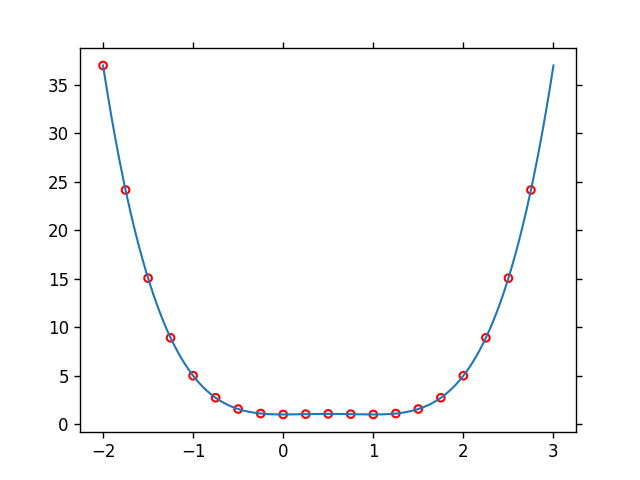
\includegraphics[scale=0.5]{plot}
			\end{center}
			
			
	\section{Genetic Programming For Classification}
			
		\subsection{Terminal Set}
			Similar to the previous problem we had two terminal nodes
			
			\begin{enumerate}
				\item \textbf{Current X:} Each problem instance is of the following form $X = \{x_1,...,x_9\}$ so we need a terminal node for each one of these features.
				
				\item \textbf{Random Number:} Like before there could be constants as part of the function. 
			\end{enumerate}
		\subsection{Function Set}			
			Like before I started with a minimal set of functions \textbf{+}, \textbf{-}, \textbf{*} and \textbf{/}. This set of functions was able to solve the problem with an acceptable amount of error (i.e. average accuracy of $94\%$ on the testing data.
			
			Then I expanded the function set to include \textbf{abs}, \textbf{sin}, \textbf{cos}, \textbf{pow}. However this dident seem to consistent or significant improvements so I decided to stick with a smaller function set as this reduced the complexity of the trees.		
			
		\subsection{Fitness Function}
			For this problem each instance describes a function $f$ which takes a set $X = \{x_1,...,x_9\}$ representing our problem instance. If $f(X) > 0$ then we give it a class of \textbf{malignant} otherwise when $f(X) \leq 0$ the instance is given a class of \textbf{benign}
			
			For each instance in our testing set we compute $f(X)$ and record a tally of the number correct. From which we compute an accuracy.
			
			To be consistent we want our fitness to be 0 when our given solution is perfect therefor we have the fitness function as $1 - accuracy$
		
		\subsection{Describe Parameters}
			\paragraph{Termination} occurs when a perfect solution is found or after 125 generations. Often the algorithm will converge after about 25 generations (i.e. Stick with a solution) but I found allowing the algorithm to run for longer sometimes yealds better solutions.
			
			\paragraph{The population size} is 1024. This will give us a more diverse population and thus more chance of finding a golbal optima.			
			
			\paragraph{The mutation probability} is $5\%$. Set to a small percentage for the same reason as in the previous example (i.e. having a probability to large can cause loss of good solutions). Also given how large our population is we dont need to rely on mutation as the main way to get diversity in our population.

			\paragraph{The crossover probability} is $90\%$
			
			\paragraph{The reproduction probability} is  $5\%$
			
			\paragraph{The maximum depth} is 5.  As allowing more nodes only provided small improvements which where not worth making the solution programs more complicated.
		
		\subsection{Classification Accuracy}
			I split the data 70:30. Giving 70\% of the examples to the training data and 30\% to testing. Not having enough samples in the training data will lead to over training and a classifier which will not generalize well. Giving the training set 70\% of samples will mean it models the underlying distribution, better than spiting the samples more equally
		
			The table below gives the fitness of the best overall individual over 10 separate runs of the algorithm		
		
			\begin{center}
				\begin{tabular}{|c|c|}
					\hline
					Training & Testing\\
					\hline
					94\% & 95\%\\
					93\% & 98\%\\
					94\% & 98\%\\
					93\% & 95\%\\
					95\% & 97\%\\
					94\% & 95\%\\
					95\% & 98\%\\
					92\% & 97\%\\
					94\% & 95\%\\
					95\% & 96\%\\
					\hline
				\end{tabular}
			\end{center}
			
			Giving us an average training accuracy of $94\%$. And an average testing accuracy of $96\%$.
			
			The training and testing accuracy are very close indicating that the classifier is well trained and isn't over fitted to the training data.
			
			Over all the data points $65.5\%$ has the class \textbf{Benign}. Assuming that we evenly split the data into training and testing then our classifier performs much better than just choosing the most common class and assigning everything that.
		
		\subsection{GP Programs}
			Over a number of runs i was able to get the following best solutions
			
			\begin{enumerate}
				\item \textbf{$((X_8 * (X_2 * (X_5 * 0.3299042674857004))) - (X_5 * 0.5596347901182992)) - X_8$} with a fitness of $0.03$ (i.e. 97\% accurate in training)	
			
				\item \textbf{$(X_7 * (X_8 * (((X_1 * X_5) * 0.3793077413934568) * 0.3793077413934568))) - X_1$} with a fitness of $0.05$ (i.e. 95\% accurate in training)
				
				\item \textbf{$((((X_3 * X_1) - X_3) - X_3) - X_3) + (X_5 - X_4$)} with a fitness of $0.06$ (i.e. 94\% accurate in training)
			\end{enumerate}
		
		\subsection{Analysis Of Program}		
			If we take the best solution we can simplify it to the following $X_8X_2X_5*0.33 - (X_5*0.55 + X_8)$. Given how our function operates ($f(X) > 0$ means that instance is malignant) this means that if $X_8X_2X_5*0.33 > X_5*0.55 + X_8$ then the instance is classified as malignant otherwise the instance is benign.
\end{document}